\chapter{Closing Remarks}
\label{cha:ClosingRemarks}

\section{Criticism}
\label{sec:Criticism}

The previous chapters addressed the advantages, benefits and possibilities of decentralized finance. But as always, there is no free lunch.
Even decentralized finance is not immune against criticism. This section provides a brief overview of a few of the most relevant issues coming
from detractors as well of a data-based evaluation whether they are valid or not.

Cryptocurrencies like Bitcoin that are using a proof-of-work algorithmn in order to achieve consensus have an extremely high power consumption.
Figure \ref{fig:BtcEnergy} shows that the Bitcoin network alone has a yearly electrical energy use of 77.78 TWh, just passing Austria with
74.1 TWh in October 2020. While this are numbers, that cannot be blandished, it is important to keep in mind that the mining algorithm on
Bitcoin is jointly responsible for its high value and is vital for the network, in order to operate in a proper and secure way.

A solution would be a proof-of-stake algorithm which is the choice of the majority of newer coins. Ethereum is already moving to proof-of-stake
as part of its update Ethereum 2.0 but that is not happening on Bitcoin anytime soon. At least 73\% of Bitcoin's electricity comes from
renewable energy sources, as investigated by researches from CoinShares \cite[p.\ 8]{CoinShares2019}. This has economical reasons. In an open
market economy, Bitcoin miners will always move to those places where energy is cheaper than anywhere else. The majority of Bitcoin mining is
done in Sichuan, China because the hydroelectrcity is very cheap in the rainy season. But there are also other attractive locations such as
Iceland and its eco-friendly geothermal energy sources.

\begin{figure}
\centering
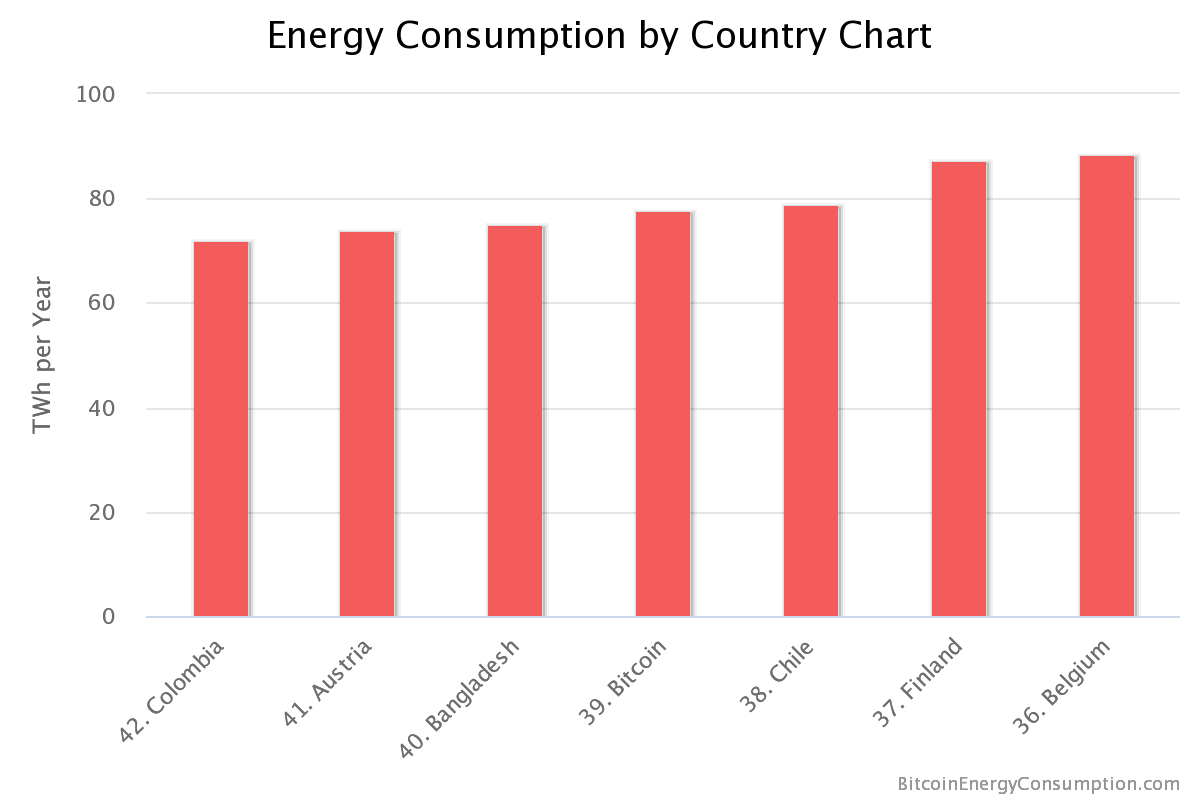
\includegraphics[width=.95\textwidth]{energy-consumption-by-co}
\caption{Bitcoin's Energy Consumption Compared to Countries \cite{Digiconomist2020}.}
\label{fig:BtcEnergy}
\end{figure}

Another popular objection is the high use of cryptocurrencies for criminalism and money laundering. While there is obviously no data about the
actual numbers of value used illegally, the majority of illicit assets still take place in fiat currencies. It is only logical, that
cryptocurrencies are the preferred choice to be used on darknet markets. But that is not a problem of the crypocurrencies themselves, as like any
technology, they are just tools which can help to achieve either good or bad things. Shifting the focus back to decentralized finance in particular,
the number of illegal activities is plummeting, as there are even more privacy focused coins like Zcash, Monero and Dash \cite[p.\ 13]{FDD2018}.

As of the arise of a lot new projects in the area of decentralized finance, some of them are exposed to ponzi schemes and similar frauds, as
fairly new projects usually are very centralized and only dispense control after time. There is no real solution for that, except enouraging
people to do their own research beforehand and by following the principle of only investing in what you understand. But even if the founders
have no bad intentions, it is still possible that users loose money due to errors in the code. This is specifically a real problem on
Ethereum, as of its turing completeness increases the risk of unconciously adding bugs to the code. DeFiChain \cite{DeFiChain}, 
a Bitcoin fork specifically adapted for decentralized financial use cases, tries to solve that problem by restricting the interaction with the
blockchain by only using few commands.

\section{Risks}
Investing in decentralized financial products has certain risks. As already mentioned in section \ref{sec:Criticism}, projects on the Ethereum
network are exposed to a high smart contract risk, due to the open design of its programming languages. Coding errors may result in loss of
funds, which are lost forever. However, the smart contract risk on Bitcoin is negleglibly low as its commands are being executed on a simple
stack machine.

The cryptocurrency market as a whole is very volatile. While this is neigher a good nor a bad thing, it definitely increases the overall risk.
Especially for new investors are exposed to make regrettable emotional decisions without doing fact-based research. Generally speaking, high
volatility is good for people with a long time horizon and who are focusing on capital gains. If people have a short time horizon or aim for
regular cashflow, they should rather avoid markets with high volatility.

A very insidious type of risk are those, which cannot be predicted. This could be scams, hacks or other so called black swan events. A black
swan is by definition an event which is extremely unlikely to happen, not predictable and it would cause potentially severe consequences.
Examples for black swan events on Bitcoin would be an evil nature of its founder Satoshi Nakamoto or a severe error in the fundamental
cryptographic algorithms.

Decentralization comes with many advantages in certain areas. But as there is a lot of freedom, people can do either good or bad things on such
an ecosystem. When thinking about tokenization, it will be possible soon to bring real world assets on a blockchain. For example, Starbucks is
already about to move their supply chain on a blockchain, where it will be completely transparent for the customer to see where the coffee beans
came from and which middlemen where involved. By scanning the QR code on the cup it will be even possible to tip the farmer on the coffee
plantage, instead of just the cashier in the store. But what if people will be tokenized too? Well, that is already reality. In 2020, basketball
player Spencer Dinwiddie tokenized his NBA contract on the Ethereum blockchain, which raised \$1.3 million \cite{Redman2020}. While this is still
quite harmless right now, there are also some dystopian scenarios like betting on a person's death.

\section{Prospective Impact}
It is inevitable that decentralized finance will continue rising in popularity in the next few years. Every new affair of a central authority
proves that again and again. We have already seen that many times in late 2020 and early 2021. Be it the tremendously high amount of new fiat
currencies being printed, blocking certain content and users on social media or by prohibiting retail investors to trade certain securities in
the GameStop short squeeze. It is all just another nail in the coffin of the traditional banking system and other centralized organizations.
But the technology is not ready yet for the mass adoption and using digital decentralized currencies on a day to day basis will certainly not
be coming in the next few years.